\documentclass{article}
%\usepackage{fullpage}

\usepackage[english,french]{babel}
\usepackage[utf8]{inputenc}
\usepackage[T1]{fontenc}

\usepackage{amsmath, amsfonts, amssymb, amsthm}
\usepackage{bbm,algorithmic,algorithm,verbatim}

\usepackage{color}
\usepackage{subcaption}
\usepackage[pdftex]{graphicx}
\graphicspath{{images/},{prebuiltimages/}}
\usepackage{epsfig}
\usepackage{ulem, stmaryrd, dsfont}

% \usepackage{mathabx} % for \vvvert ||| |||
\usepackage{../sty/scribe}
\usepackage{../sty/shortcuts_js}


%%%%%%%%%%%%%%%%%%%%%%%%%%%%%%%%%%%%%%%%%%%%%%%%%%%%%%%%%%%%%%%%%%%%%%%%%%%%%%%
% Hyperlinks
%%%%%%%%%%%%%%%%%%%%%%%%%%%%%%%%%%%%%%%%%%%%%%%%%%%%%%%%%%%%%%%%%%%%%%%%%%%%%%%

\PassOptionsToPackage{hyphens}{url}
\usepackage[pdftex,linkcolor=test,citecolor=vsomb_col,
colorlinks=true,pagebackref,bookmarks=true,plainpages=true,
urlcolor=fb_col]{hyperref}
\usepackage{cleveref}


\begin{document}
\sloppy
\lecture{HMMA237}{Complement de Schur et applications}{Joseph Salmon}{nomeleve1 et nomeleve2}


%%%%%%%%%%%%%%%%%%%%%%%%%%%%%%%%%%%%%%%%%%%%%%%%%%%%%%%%%%%%%%%%%%%%%%%%%%%%%%%
%%%%%%%%%%%%%%%%%%%%%%%%%%%%%%%%%%%%%%%%%%%%%%%%%%%%%%%%%%%%%%%%%%%%%%%%%%%%%%%
\section{Introduction}
\label{sec:introduction}
%%%%%%%%%%%%%%%%%%%%%%%%%%%%%%%%%%%%%%%%%%%%%%%%%%%%%%%%%%%%%%%%%%%%%%%%%%%%%%%
%%%%%%%%%%%%%%%%%%%%%%%%%%%%%%%%%%%%%%%%%%%%%%%%%%%%%%%%%%%%%%%%%%%%%%%%%%%%%%%


%%%%%%%%%%%%%%%%%%%%%%%%%%%%%%%%%%%%%%%%%%%%%%%%%%%%%%%%%%%%%%%%%%%%%%%%%%%%%%%
\subsection{Filtre de Kallman}
%%%%%%%%%%%%%%%%%%%%%%%%%%%%%%%%%%%%%%%%%%%%%%%%%%%%%%%%%%%%%%%%%%%%%%%%%%%%%%%


Part of the elements in this part can be found in \cite{Hiriart-Urruty_Lemarechal93,Hiriart-Urruty_Lemarechal93b}
\begin{definition}[Strong convexity]
A function $f$ is said $\lambda$-strongly convex if the function
$\left(f - \lambda \norm{\cdot}^2\right)$ is convex.
\end{definition}

\begin{remark}
The norm used in this document is always the Euclidean norm: $\norm{\,\cdot\,} = \norm{\,\cdot\,}_2$.
\end{remark}


\begin{proposition}
The function $f$ is $\lambda$-strongly convex if and only if $
\forall w_1 w_2, \forall \alpha \in [0,1]:$
\begin{equation}\label{eq:strong}
f\left(\alpha w_1 + (1-\alpha) w_2\right)
\leq
\alpha f(w_1) + (1-\alpha) f(w_2) - \lambda \alpha (1-\alpha) \norm{w_1-w_2}^2
\end{equation}
\end{proposition}


We will then use $w^{(\alpha)}$ to denote $\alpha w_1 + (1-\alpha) w_2$.

\begin{proof}
Firstly, we remark that for all $\alpha \in [0,1]$,
$$ \norm{w^{(\alpha)}}^2 = \alpha^2\norm{w_1}^2 + (1-\alpha)^2\norm{w_2}^2 + 2 \alpha (1-\alpha) \scal{w_1}{w_2}$$
Then, we prove the equivalence of the two statements.
$f$ is strongly convex if and only if the following inequality is valid for all $\alpha \in [0,1]$.
\begin{equation*}
f(w^{(\alpha)}) - \lambda \norm{w^{(\alpha)}}^2 \leq  \alpha f(w_1) + (1-\alpha) f(w_2) - \lambda \left( \alpha \norm{w_1}^2 + (1-\alpha)\norm{w_2}^2\right)\\
\end{equation*}
Then, by replacing $\norm{w^{(\alpha)}}$ by its expression, we obtain:
\begin{equation*}
f(w^{(\alpha)}) \leq \alpha f(w_1) + (1-\alpha) f(w_2) -
 \lambda \left( \left(\alpha-\alpha^2\right) \norm{w_1}^2 +\left((1-\alpha)-(1-\alpha)^2\right)\norm{w_2}^2 + 2 \alpha(1-\alpha)\scal{w_1}{w_2}\right)
\end{equation*}
By reducing and factorizing, we get the following inequalities
\begin{equation*}
f(w^{(\alpha)}) \leq \alpha f(w_1) + (1-\alpha) f(w_2) -
 \lambda \alpha (1-\alpha) \left( \norm{w_1}^2 +\norm{w_2}^2 - 2 \scal{w_1}{w_2}\right)
\end{equation*}
\end{proof}

\begin{figure}[htbp]
  \centering
  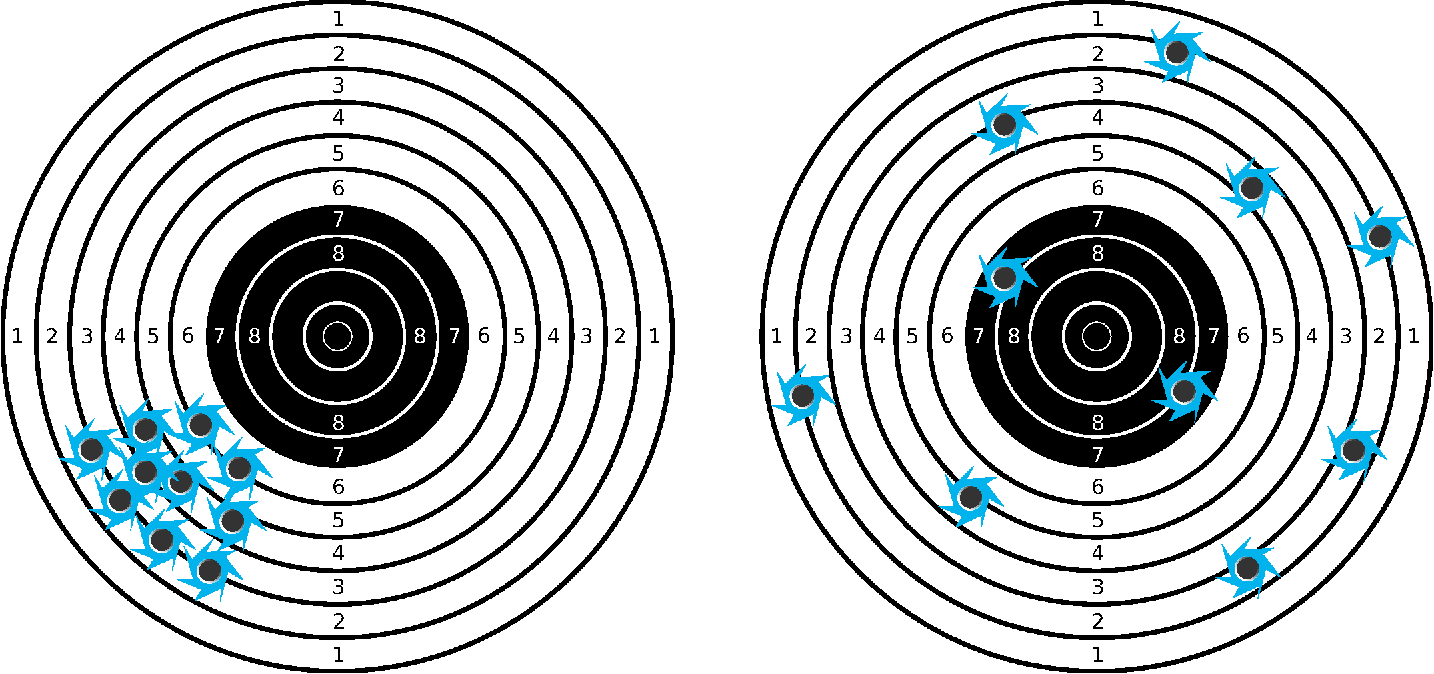
\includegraphics[width=0.95\textwidth]{cible_biais_variance}
  \caption{A figure explaining the bias/variance tradeoff}
  \label{fig:my_nice_figure}
\end{figure}


%%%%%%%%%%%%%%%%%%%%%%%%%%%%%%%%%%%%%%%%%%%%%%%%%%%%%%%%%%%%%%%%%%%%%%%%%%%%%%%
%%%%%%%%%%%%%%%%%%%%%%%%%%%%%%%%%%%%%%%%%%%%%%%%%%%%%%%%%%%%%%%%%%%%%%%%%%%%%%%
\section{Pour aller plus loin sur ce thème}
\label{sec:pour_aller_plus_loin_sur_ce_theme}
%%%%%%%%%%%%%%%%%%%%%%%%%%%%%%%%%%%%%%%%%%%%%%%%%%%%%%%%%%%%%%%%%%%%%%%%%%%%%%%
%%%%%%%%%%%%%%%%%%%%%%%%%%%%%%%%%%%%%%%%%%%%%%%%%%%%%%%%%%%%%%%%%%%%%%%%%%%%%%%

Parmi les livres intéressant on notera aussi:
\cite{Boyd_Vandenberghe04}, \cite{Beck17}


%%%%%%%%%%%%%%%%%%%%%%%%%%%%%%%%%%%%%%%%%%%%%%%%%%%%%%%%%%%%%%%%%%%%%%%%%%%%%%%
\bibliographystyle{alpha}
\bibliography{../biblio/references_all}
%%%%%%%%%%%%%%%%%%%%%%%%%%%%%%%%%%%%%%%%%%%%%%%%%%%%%%%%%%%%%%%%%%%%%%%%%%%%%%%

\end{document}